\chapter{Contribution}
\label{sec:contribution}

In the following chapter, contribution during Master Thesis is presented.
As result, a GNN can be presented which is called \textit{GAT-Denoiser}.
It main components and the overall architecture, will be explained in the current chapter.

The focus during practical part was on classical computed tomography in 2D but
can be generalized to cryo-EM and 3D.


\paragraph{Goal}
As introduced in chapter~\ref{sec:imaging}, molecular imaging methods computed tomography and cryo-EM are the problems
to approach. Further, the high-noise regime is the domain of interest, to be precise SNR between $[-20, 0]$.

For a given set of observations (many sinograms or micrographs), a GNN will be trained, such that
it enables denoising of observations which are expected to have better reconstruction results.

To recap from section~\ref{sec:graphConstruction}, our graph from molecular-imaging observation
will have single observations as nodes (one horizontal line of the sinogram). 
As $\theta$ is fixed, angle corresponding to each single observation is known. 
Based on these angles, neighbourhing nodes can be connected.


\begin{tcolorbox}[colback=red!5!white,colframe=red!75!black]
  To start solving the problem, an algorithm was designed to work with computed tomography, further
  projection angles are assumed to be known and $\theta$ was defined as equally spaced points on the unit-circle. \\

  Therfore, in the following chapters the main focus will be on computed tomography. 
  But, the concept of the algorithm would work in 3D, so for cryo-EM as well.
\end{tcolorbox}



\section{Components}
In the following section, the components of the presented algorithm is introduced, which is called \textit{GAT-Denoiser}. 
GAT-Denoiser is a graph neural network and the main component is a GAT. 
The main idea of GAT-Denoiser is to enable denoising of observations:
\begin{equation}
  \text{GAT-Denoiser} (\cdot) : L^2(\tilde{\Omega}) \to  L^2(\tilde{\Omega}) , y \mapsto \text{GAT-Denoiser} (y) 
\end{equation}

The GAT is expected to denoise observation signal with its neighbours by averaging. 
Further, convolution is added to denoise single observations.

But the main goal is to get the best possible reconstruction from original object $x$ based from noisy observation $y$ 
and not just denoise observation $y$ to approximate noiseless observation $p$:

\begin{equation}
  x \approx   Recon \left( \text{GAT-Denoiser} \left( y \right) \right)
\end{equation}

Therefore, an end-to-end learning approach is used where quality of reconstruction is 
compared in the loss during GAT-Denoiser training, which is expected to perform better than 
only optimizing denoising of observations.

\paragraph{Fixed projection angles}
As already mentioned, projection angles are assumend to be fixed and equally spaced on the unit-circle.
This assumption is pretty strong, but good to start with developing an algorithm.

\begin{tcolorbox}[colback=red!5!white,colframe=red!75!black]
  For our GNN, this means that graph is fixed. A K-NN graph can be built from points, equally spaced on the unit-circle.
  As the signal of our observations is assumed to process the low-dimensional manifold.
\end{tcolorbox}


In the following, components of GAT-Denoiser are explained in more detail.


\subsection{Graph Attention Networks}
As mentioned in section~\ref{sec:graph_depp_learning}, GAT is an extension to GCN and 
adds attention (or weights) to neighbours for learning a new node feature representation. 
Again, the topology of the graph will no change but weighted averaging over the neighbourhood 
will take place and this is what in denoising is a good idea.

\paragraph{Single Layer}
Input of a single GAT layer are node features $h = \{ h_1, h_2, \dots , h_N \} \in \mathbb{R}^F$, 
where $N$ is the number of nodes and $F$ the number of features per node. 
The layer will map input to output, which can potentially have different dimensions: 
$h^{\prime} = \{ h_1^{\prime}, h_2^{\prime}, \dots, h_N^{\prime} \} \in \mathbb{R}^{F^{\prime}} $

As is other GNNs, input features are initially 
linearly transformed and parametrized by a learnable weight matrix $W \in \mathbb{R}^{F^{\prime} \times F}$.
This allows to add enough expressiveness to the neural network and weights are learned during training.

Further, attention coefficiants are computed, which indicate the importance of node $j$ to node $i$:

\begin{equation}
  e_{ij} = a(Wh_i, Wh_j),
\end{equation}

with $a$ as the shared attentional meachanism $a : \mathbb{R}^{F^{\prime}} \times \mathbb{R}^{F^{\prime}} \mapsto \mathbb{R}$.
But how to define the attentional mechanism? 
\citet{GAT} proposed to use a single-layer feedforward neural network, paremetrized by a weight vector $a \in \mathbb{R}^{2F^{\prime}}$
and LeakyReLu as activation function, which is good to start with.
 
Coefficients $e$ need to be normalized, such that all attention coefficient of one node sum up to 1 and therefore are comparable nicely across nodes.
Therefore, softmax is used as normalization and normalized attention coefficient are defined as:
\begin{equation}
  \alpha_{ij} = softmax_j(e_{ij})
\end{equation}


Finally, the new node embedding is calculated as:

\begin{equation}
  h_i^{\prime} = \sigma \left( \sum_{j \in \mathcal{N}_i} \alpha_{ij} W h_j \right),
\end{equation}

with $\sigma$ as some arbitrary activation function.

\paragraph{Multi-Head attention}
Motivated by \citet{transformer}, multi-head attention can be beneficial to stabilize the learning process.
Therefore, not only single weight matrix is learned but it is splitted up in several parts, 
all learned individually:

\begin{equation}
  h_i^{\prime} = \bigparallel^K_{k=1} \sigma \left(\sum_{j \in \mathcal{N}_i} \alpha_{ij}^k W^k h_j \right),  
\end{equation}

where $\parallel$ corresponds to concatenation, $\alpha_{ij}^k$ the $k$-th attention mechanism and $W^k$ the linear
transformations weight matrix. The final output consists of $KF^{\prime}$ output features.

\paragraph{Last layer:}
If working with multiple heads, in the last layer of our neural network, concatenation is not the desired 
way to prepare for output and therefore, averaging instead of concatenation is used.

\subsection{Convolution}
The second key component of our GAT-Denoiser is convolution.
Convolution is an important part in Signal Processing, if not the most important one.
It allows to average an incoming signal, further, it is very popular in computer vision.

\begin{equation}
  y \star k = \tilde{y}
\end{equation}

To do convolution, a kernel needs to be defined.
This kernel will then slide over the signal and will computed the dot product with the filter weights.



Convolution will be used in GAT-Denoiser. 
The GAT will be responsible to average over observation neighbours, but single observations will
not be averaged by the GAT. 
Therefore, convolution is added and is responsible to denoise single observations
before averaging over neighbourhood with GAT.

\subsection{U-Net}
U-Net can boost the performance of computed tomography reconstruction.
It is an convolutional neural network, which is well suited for image segmentation in different domains.
\cite{unet-tomography} showed great success for biomedial image segmentation.

The neural network architecture consists of two main path, the contracting path and the expansive path,
resulting in a U-shape, and therefore the naming \cite{unet-tomography}.


\section{Architecture}
Now, all individual components are introduced, the overall architecture can be defined.

\paragraph{GAT contribution:}

\paragraph{Convolution contribution:}

\paragraph{End-to-end learning contribution:}


\begin{figure}[h]
  \centering
  \label{fig:architecture-overall}
  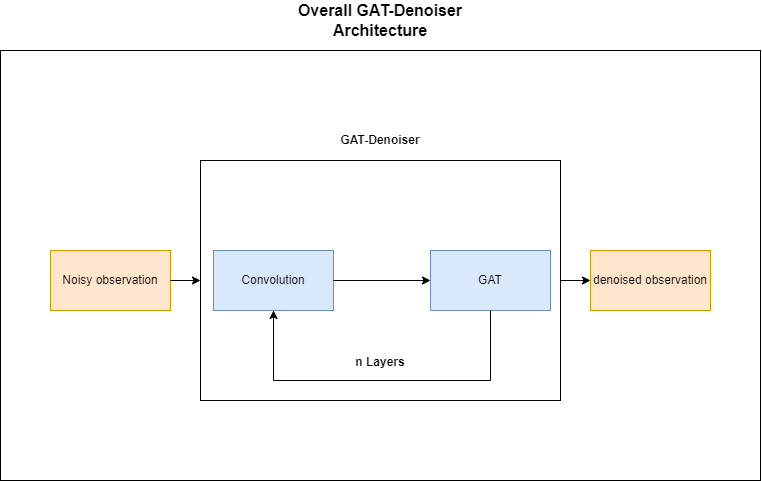
\includegraphics[width=0.6\textwidth]{Overall_final_Architecture.drawio.png}
  \caption{Overall GAT-Denoiser architecture}
\end{figure}


\subsection{Layers}
\textbf{TODO: Add detailed illustration}

\begin{figure}[h]
  \centering
  \label{fig:architecture-detailed}
  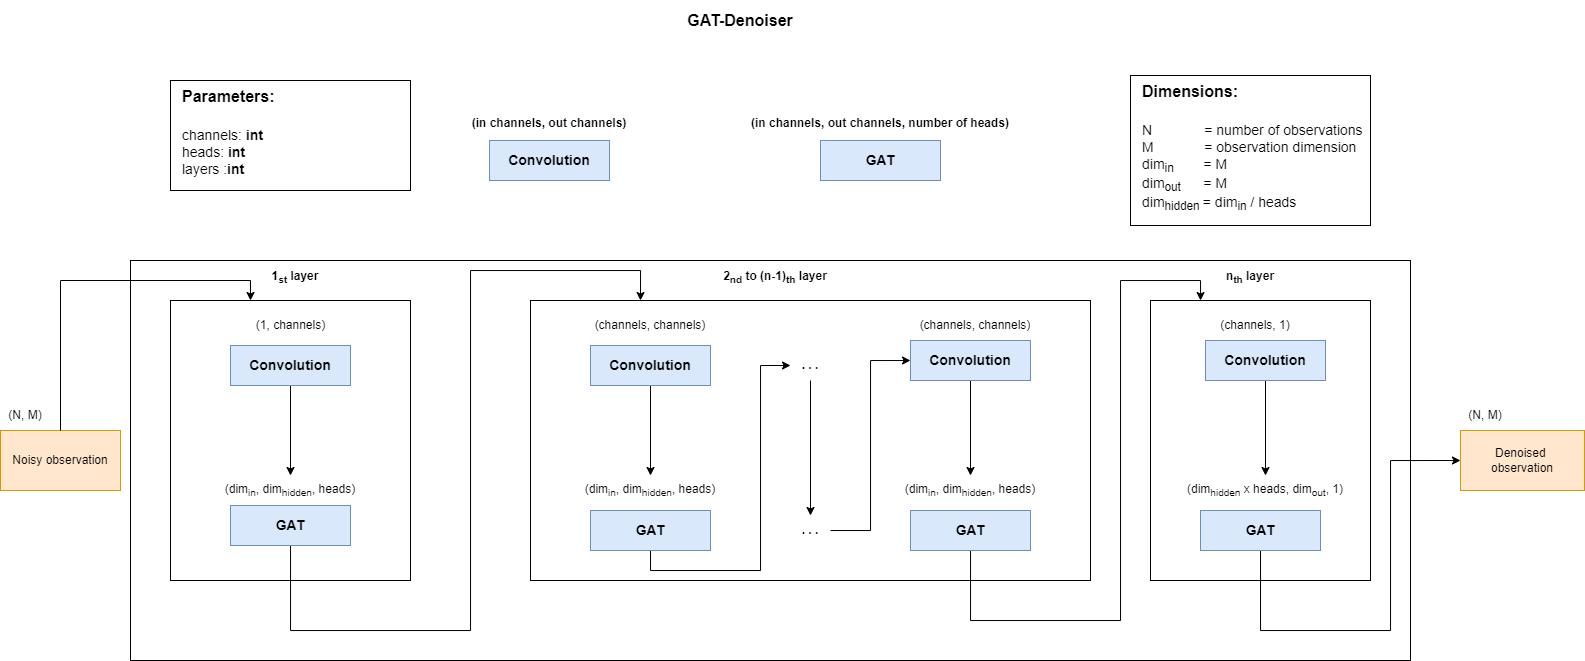
\includegraphics[width=0.8\textwidth]{GAT_Architecture_Detail.drawio.png}
  \caption{Overall GAT-Denoiser architecture}
\end{figure}


\subsection{Training:}

\paragraph{Loss:}

\begin{equation}
  \mathcal{L} = || x_i - Recon ( \text{GAT-Denoiser}(A(x_i, \theta, s) + \eta)) ||^2_2
\end{equation}


\begin{figure}[h]
  \centering
  \label{fig:pipeline-overall}
  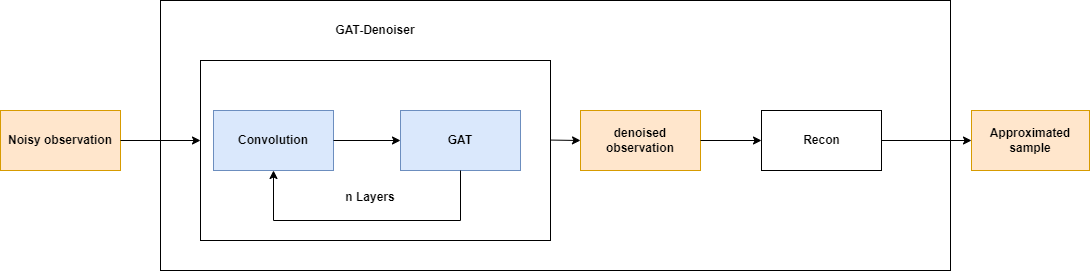
\includegraphics[width=0.8\textwidth]{Overall_GAT-Denoiser_Pipeline.drawio.png}
  \caption{Overall GAT-Denoiser architecture}
\end{figure}

\paragraph{U-Net:}
Therefore, U-Net will be jointly used with FBP as reconstruction. For that to work, U-Net needs to be 
first trained with the dataset and the learned model can be be pluged in to GAT-Denoiser.
It is expected, than the pre trained model of U-Net can be join
\textbf{TODO: Pre traing U-Net to further boost quality of FBP.}
Even train it jointly with gat.





